\chapter{TẠO THƯ VIỆN SCHEMATIC VÀ PCB 3D}
    \section{Trình tự tạo thư viện schematic}
        Bước 1: Chọn File/New/Library để tạo thư viện mới.
        \begin{figure}[H]
            \centering
            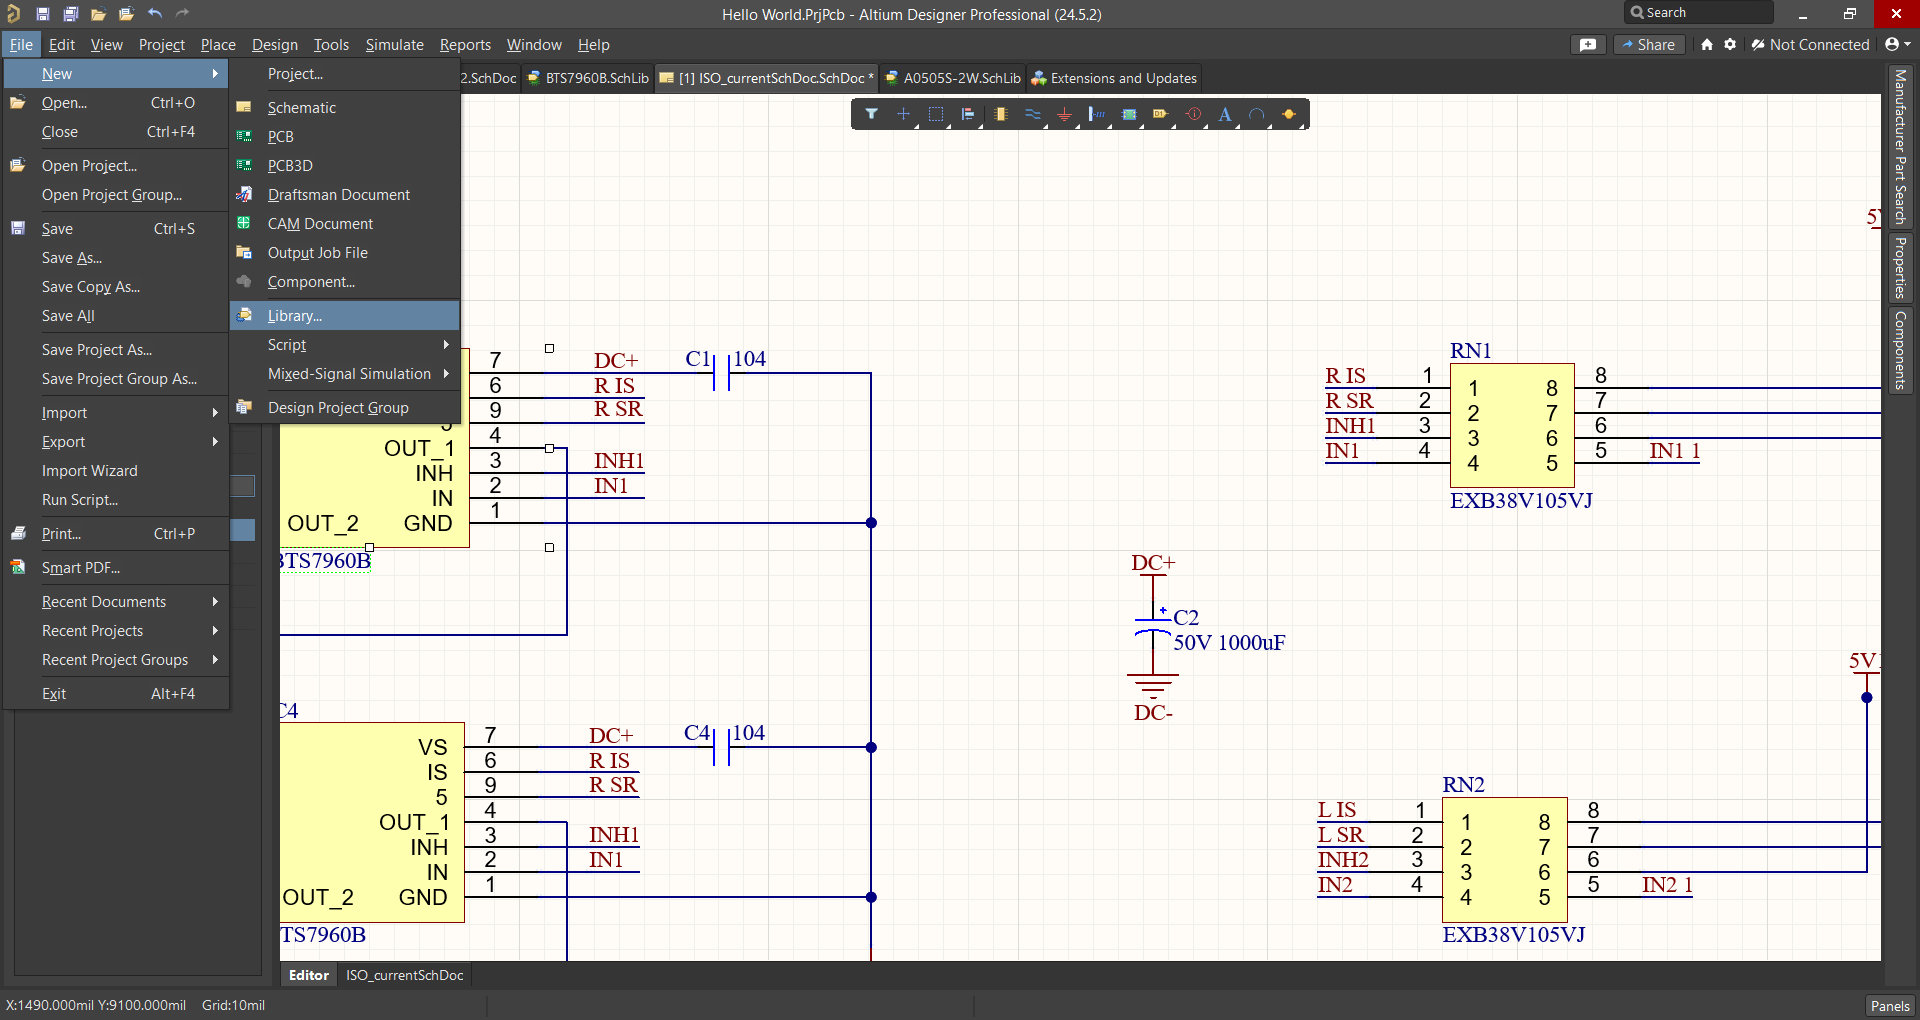
\includegraphics[width=1\textwidth]{pictures/ch3.1.png}
        \end{figure}
        Bước 2: Chọn Schematic Library và nhấn Create.
        \begin{figure}[H]
            \centering
            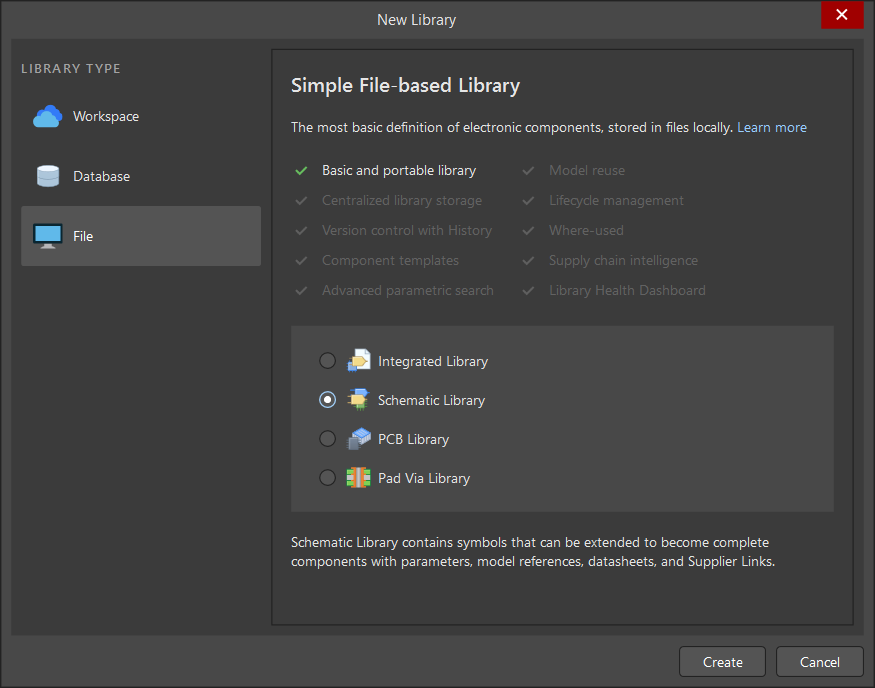
\includegraphics[width=0.8\textwidth]{pictures/ch3.2.png}
        \end{figure}
        Bước 3: Vẽ khối và đặt các chân theo hướng dẫn của datasheet.
        \begin{figure}[H]
            \centering
            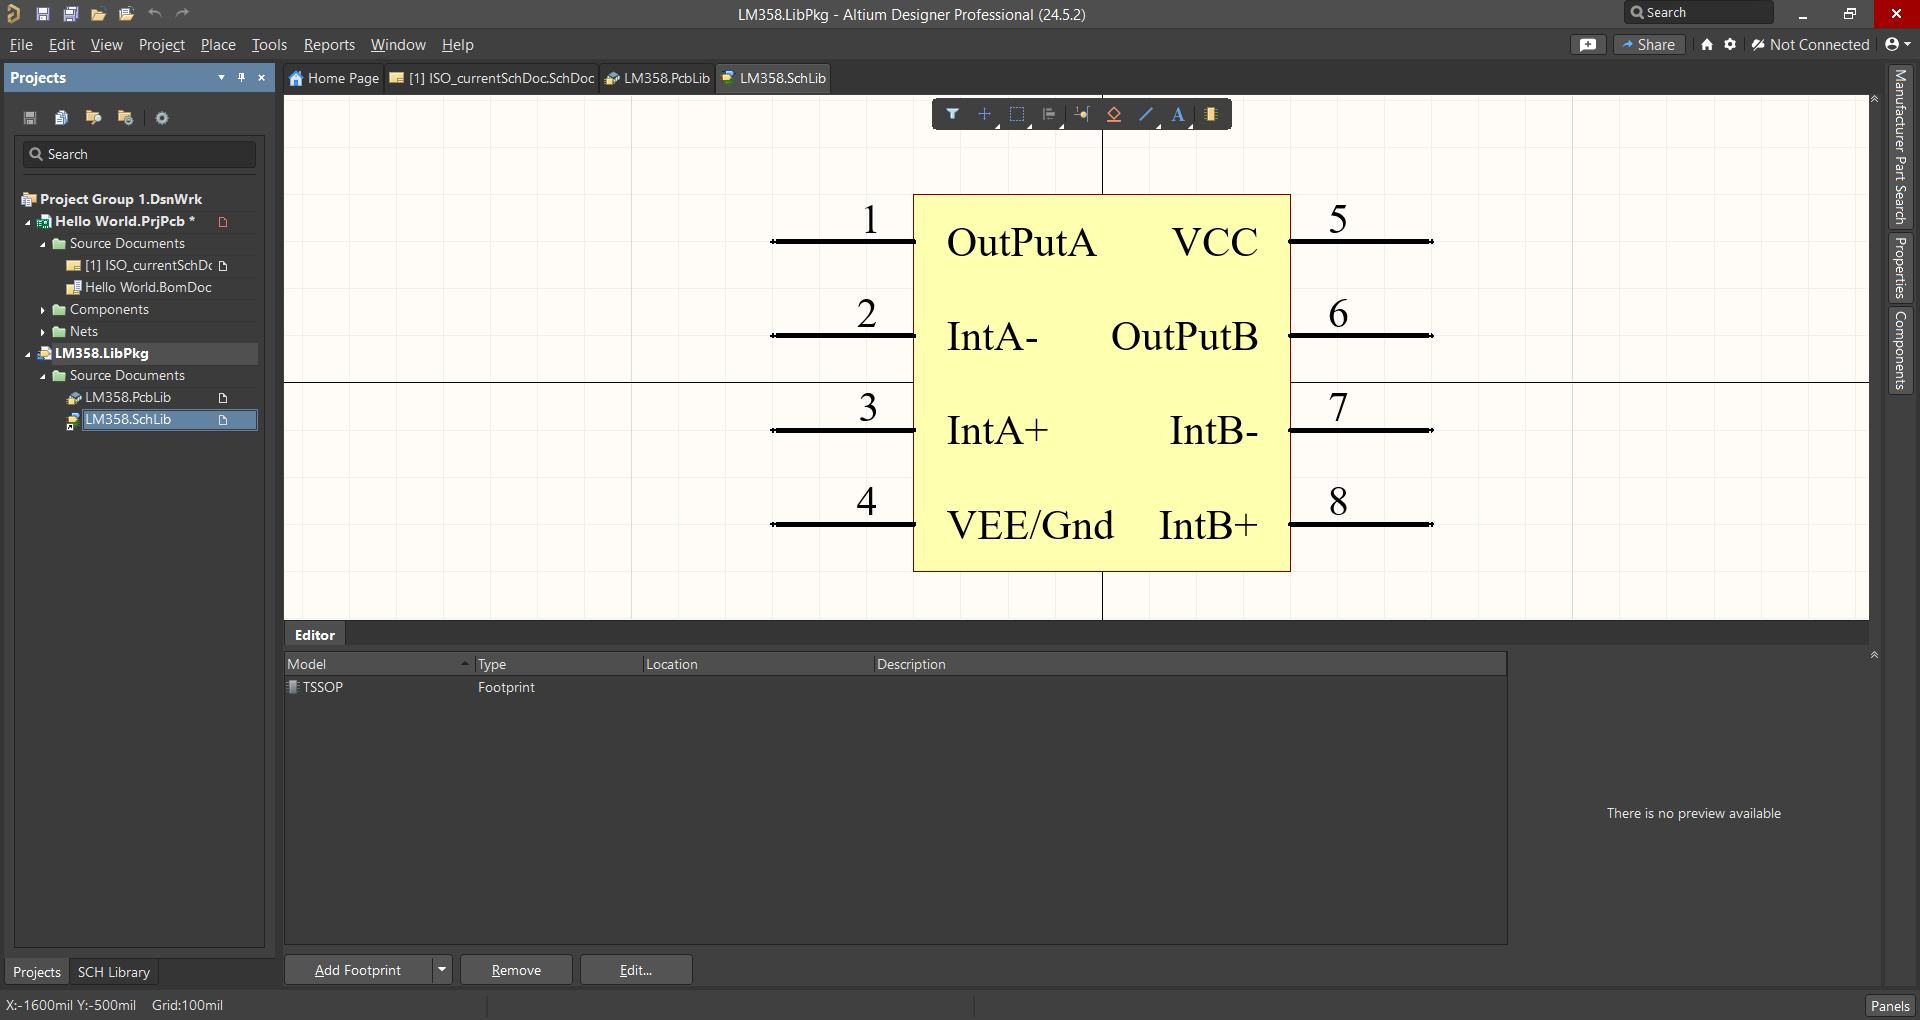
\includegraphics[width=1\textwidth]{pictures/ch3.3.png}
        \end{figure}
        Bước 4: Đặt tên cho thư viện và lưu lại.\\
    \section{Trình tự tạo thư viện PCB }
        \textbf{Ví dụ: Tạo thư viện fPCB 3D cho LM358 SOP8.}\\
        Bước 1: Chọn File/New/Library để tạo thư viện mới.\\
        Bước 2: Chọn PCB Library và nhấn Create.
        \begin{figure}[H]
            \centering
            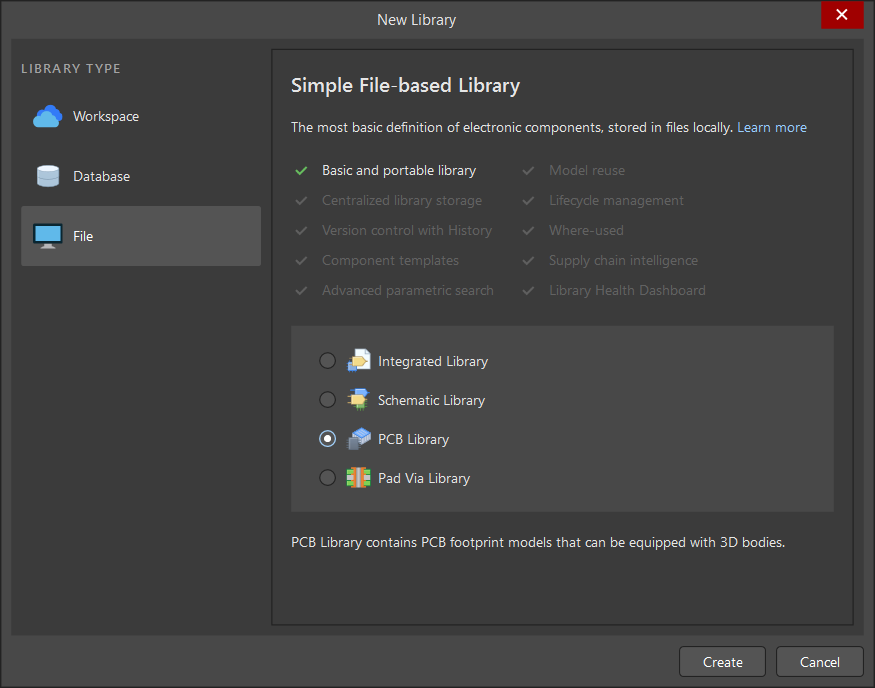
\includegraphics[width=0.7\textwidth]{pictures/ch3.4.png}
        \end{figure}
        Bước 3: Chọn Tools/IPC Compliant Footprint Wizard/Next.
        \begin{figure}[H]
            \centering
            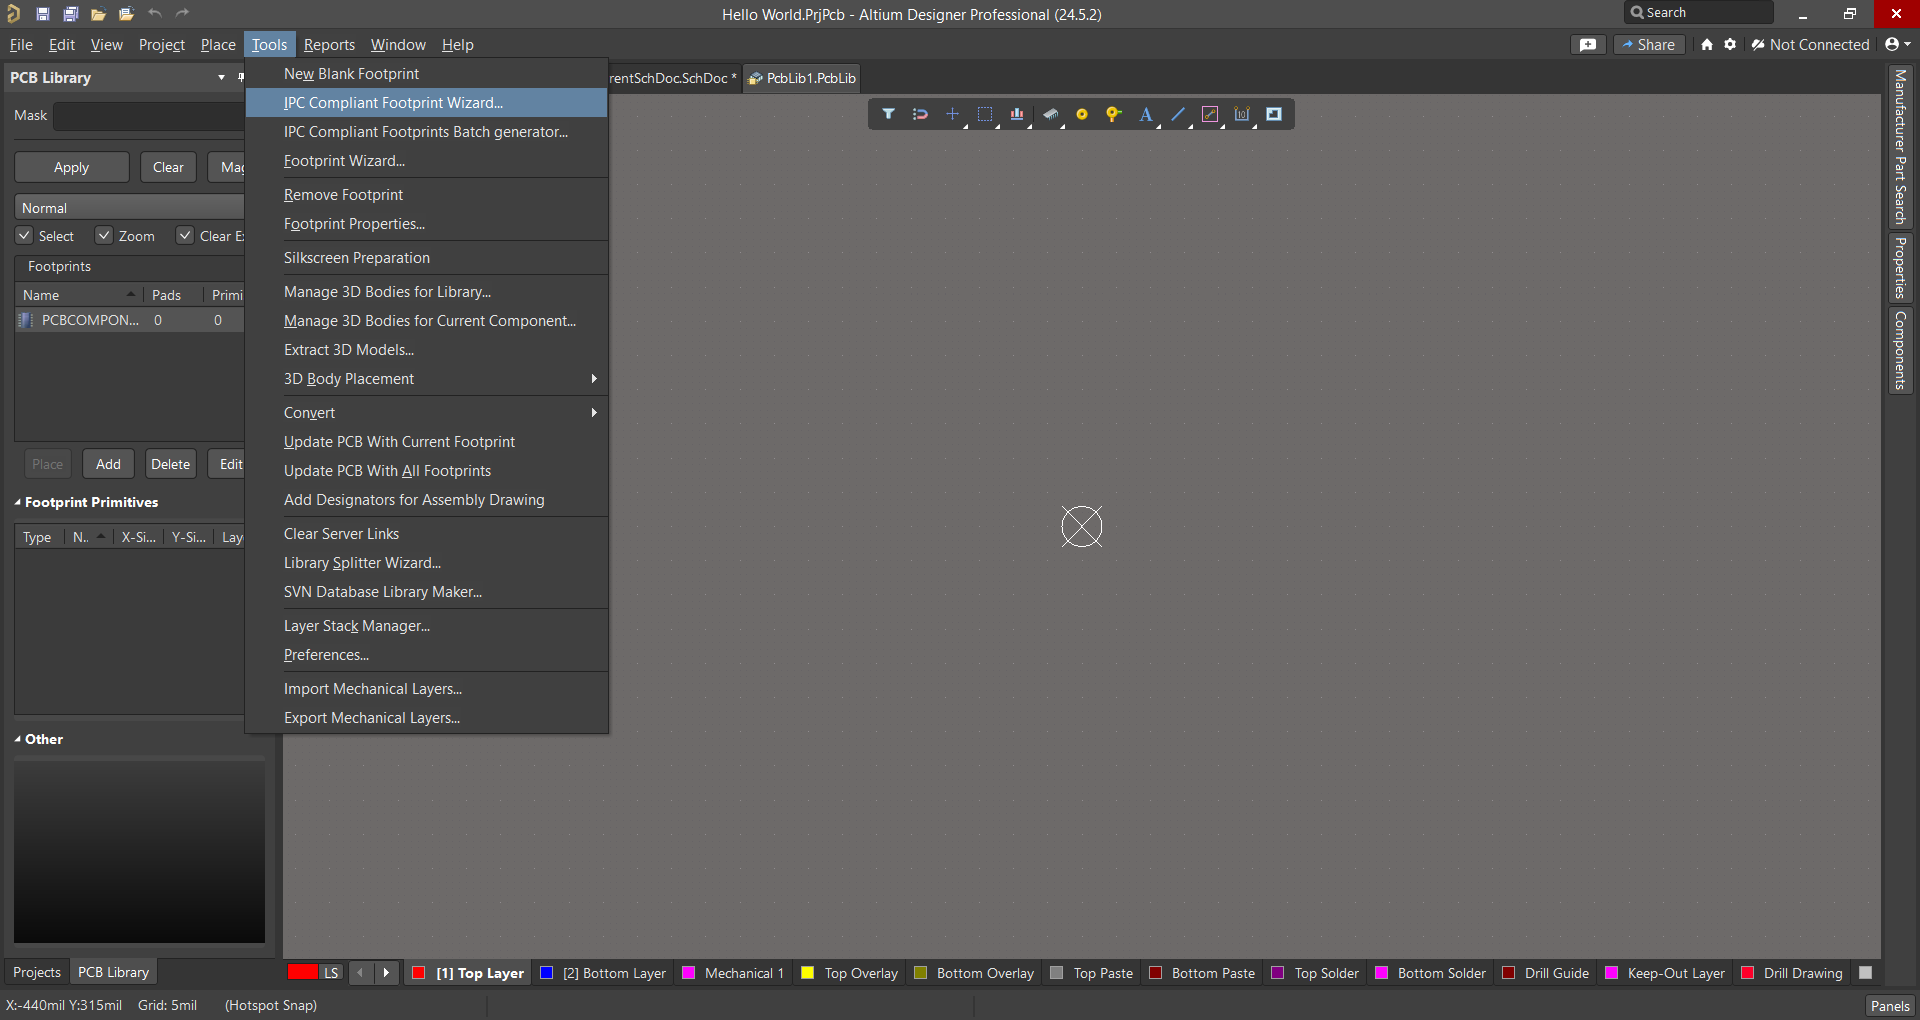
\includegraphics[width=1\textwidth]{pictures/ch3.5.png}
        \end{figure}
        Bước 4: Chọn kiểu chân SOP/TSOP và nhấn NEXT.
        \begin{figure}[H]
            \centering
            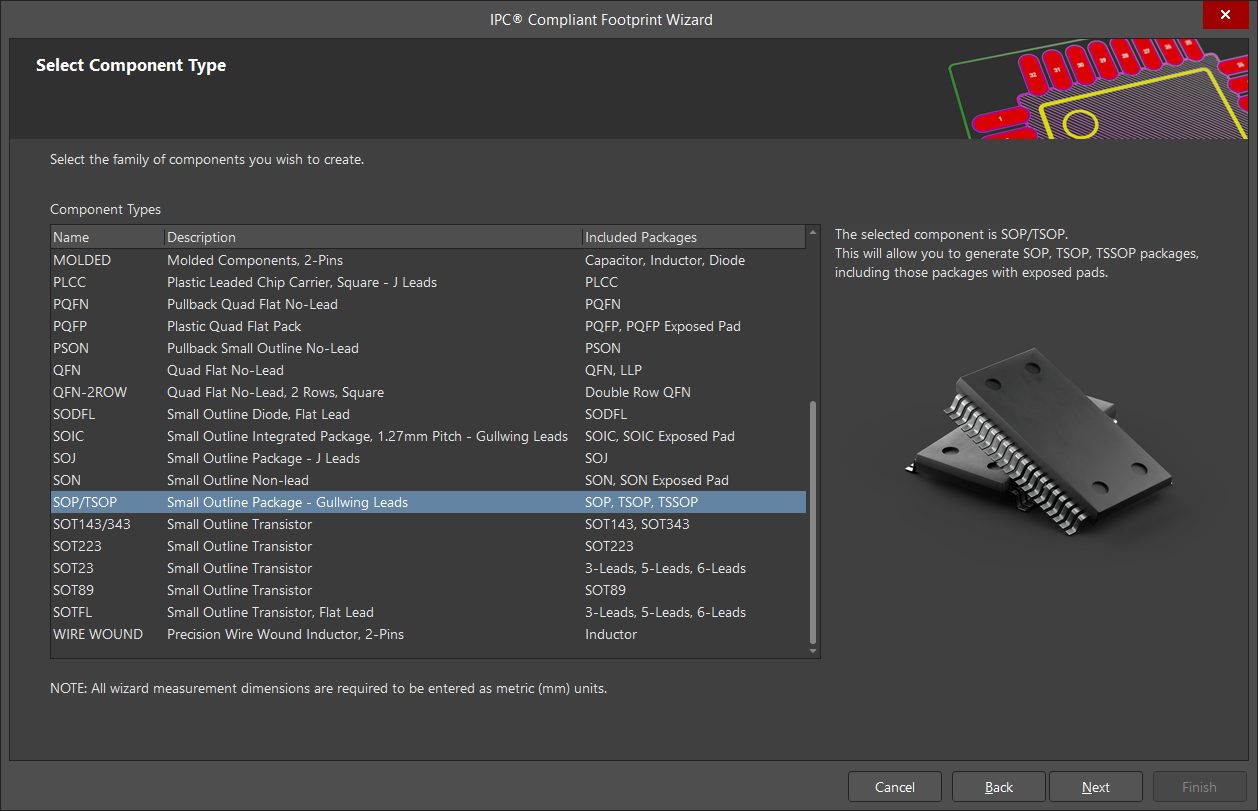
\includegraphics[width=1\textwidth]{pictures/ch3.6.png}
        \end{figure}
        \cleardoublepage
        Bước 5: Đọc datasheet của linh kiện để tìm các thông số thiết kế.
        \begin{figure}[H]
            \centering
            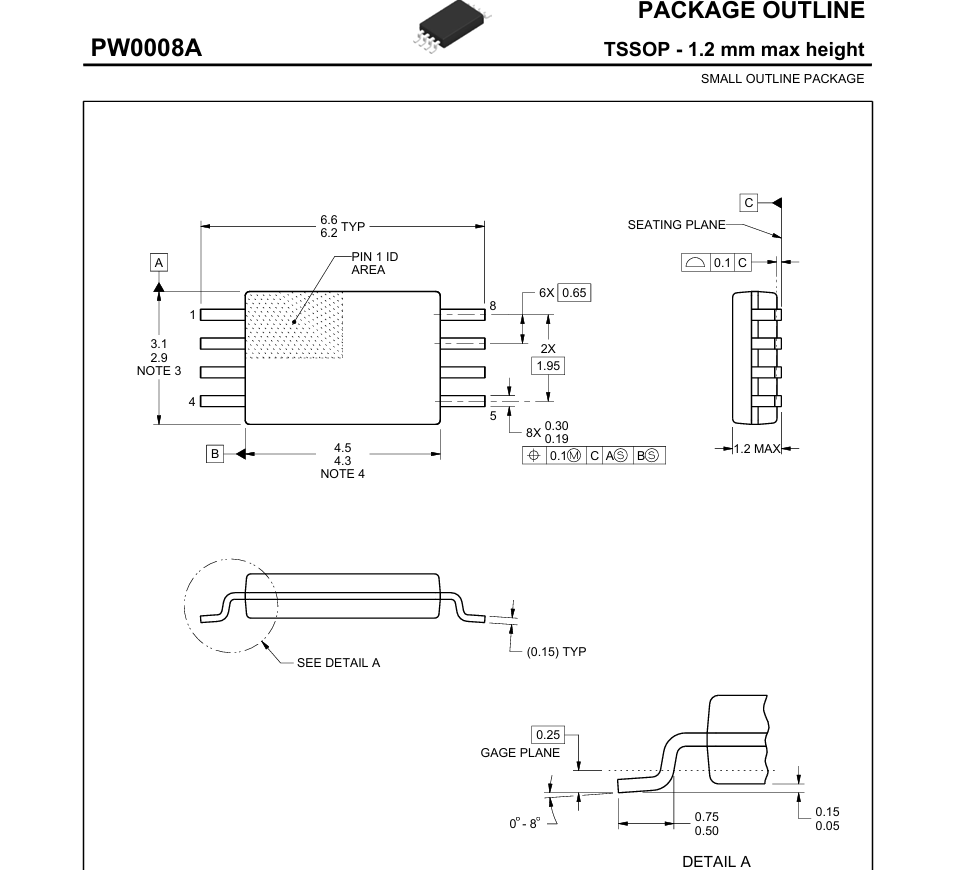
\includegraphics[width=0.9\textwidth]{pictures/ch3.7.png}
        \end{figure}
        Bước 6: Nhập các thông số vào các ô tương ứng và nhấn NEXT.
        \begin{figure}[H]
            \centering
            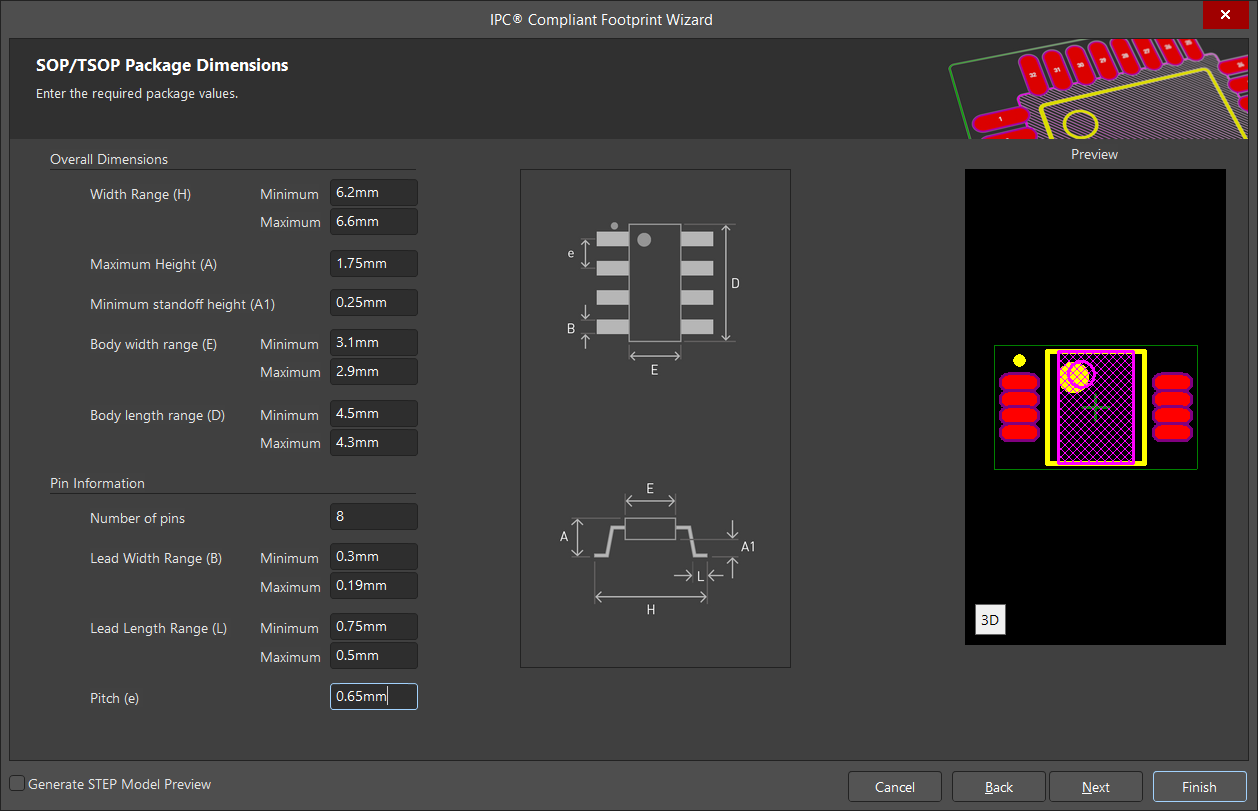
\includegraphics[width=0.8\textwidth]{pictures/ch3.8.png}
        \end{figure}
        Bước 7: Tiếp tục nhấn NEXT cho đến khi đến màn hình lưu và đặt tên.
        \begin{figure}[H]
            \centering
            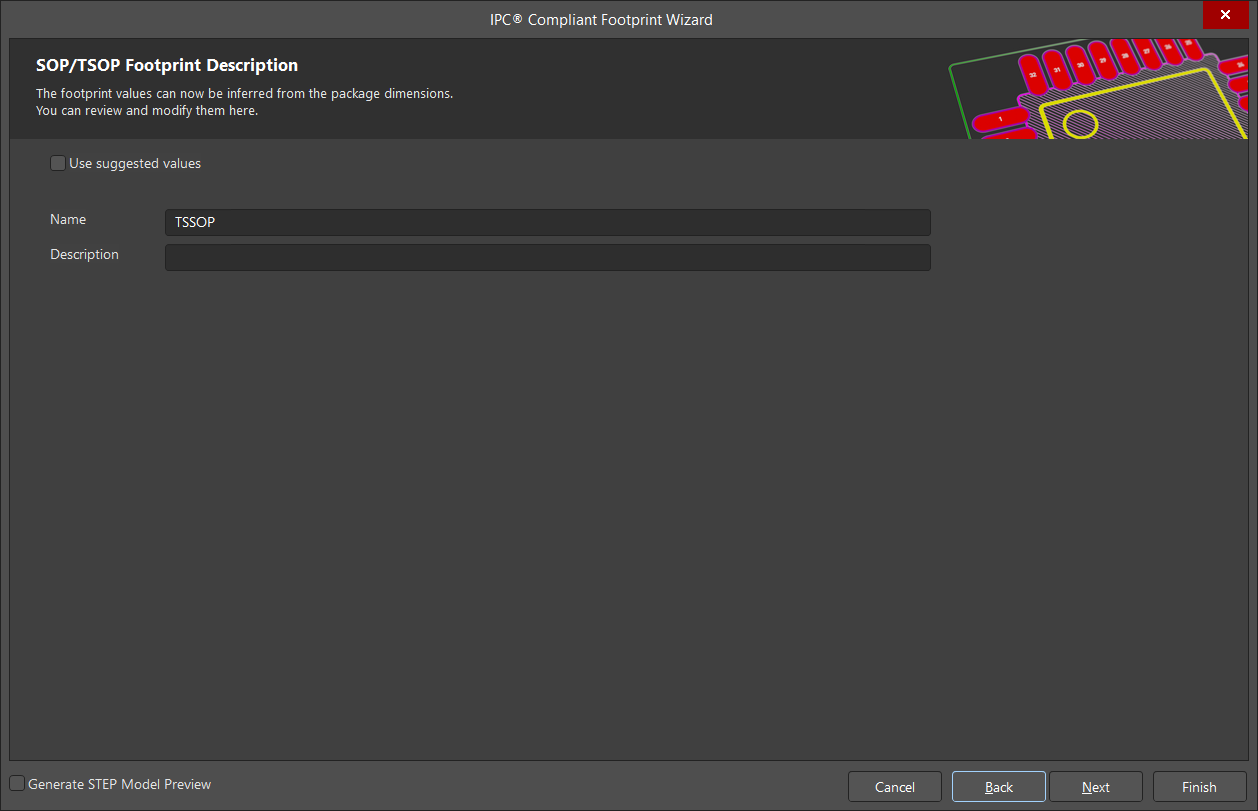
\includegraphics[width=1\textwidth]{pictures/ch3.9.png}
        \end{figure}
        Bước 8: Chọn Produce 3D/STEP model nhấn NEXT và FINISH.
        \begin{figure}[H]
            \centering
            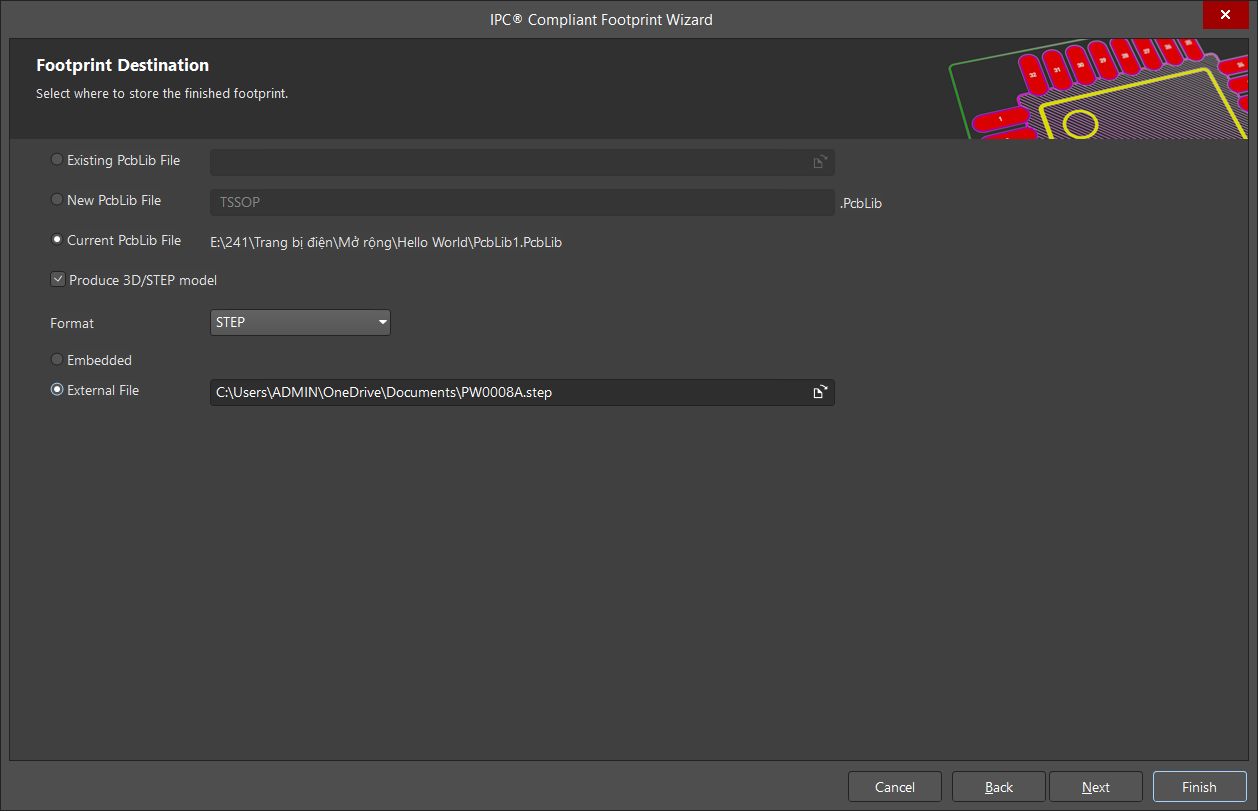
\includegraphics[width=1\textwidth]{pictures/ch3.10.png}
        \end{figure}
        \cleardoublepage
        Bước 9: Hoàn thành việc tạo thư viện footprint cho linh kiện LM358 SOP8.
        \begin{figure}[H]
            \centering
            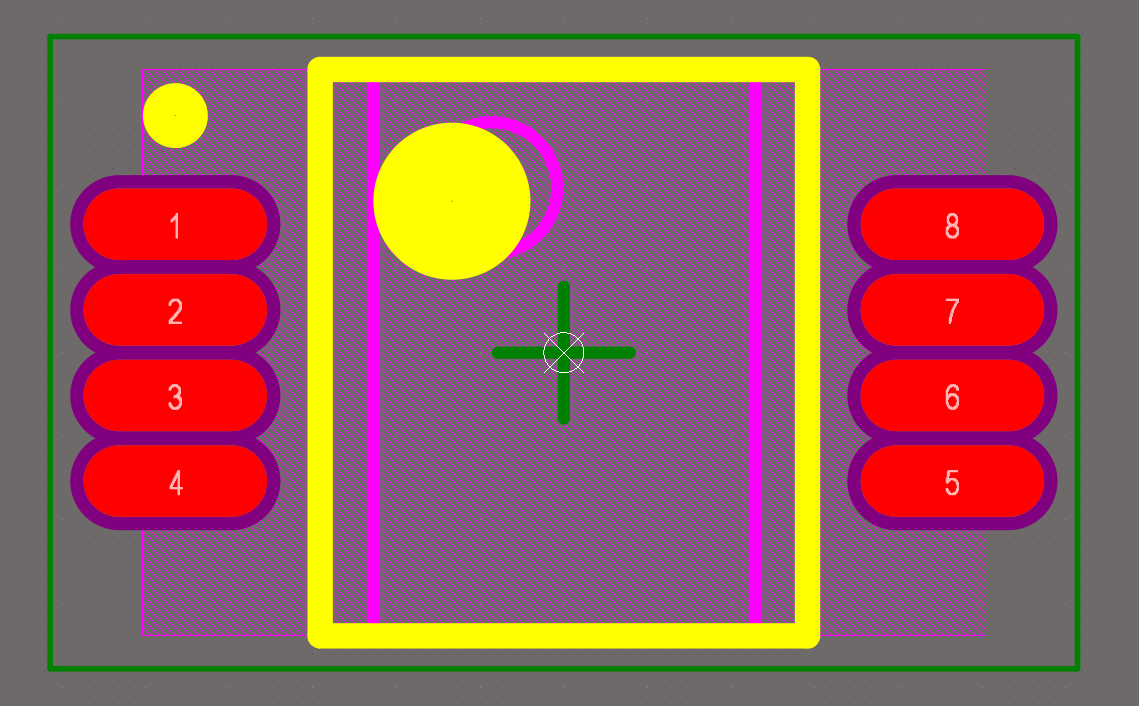
\includegraphics[width=0.9\textwidth]{pictures/ch3.11a.png}
            \caption{Footprint LM358 SOP8 vừa tạo} 
        \end{figure}
        \begin{figure}[H]
            \centering
            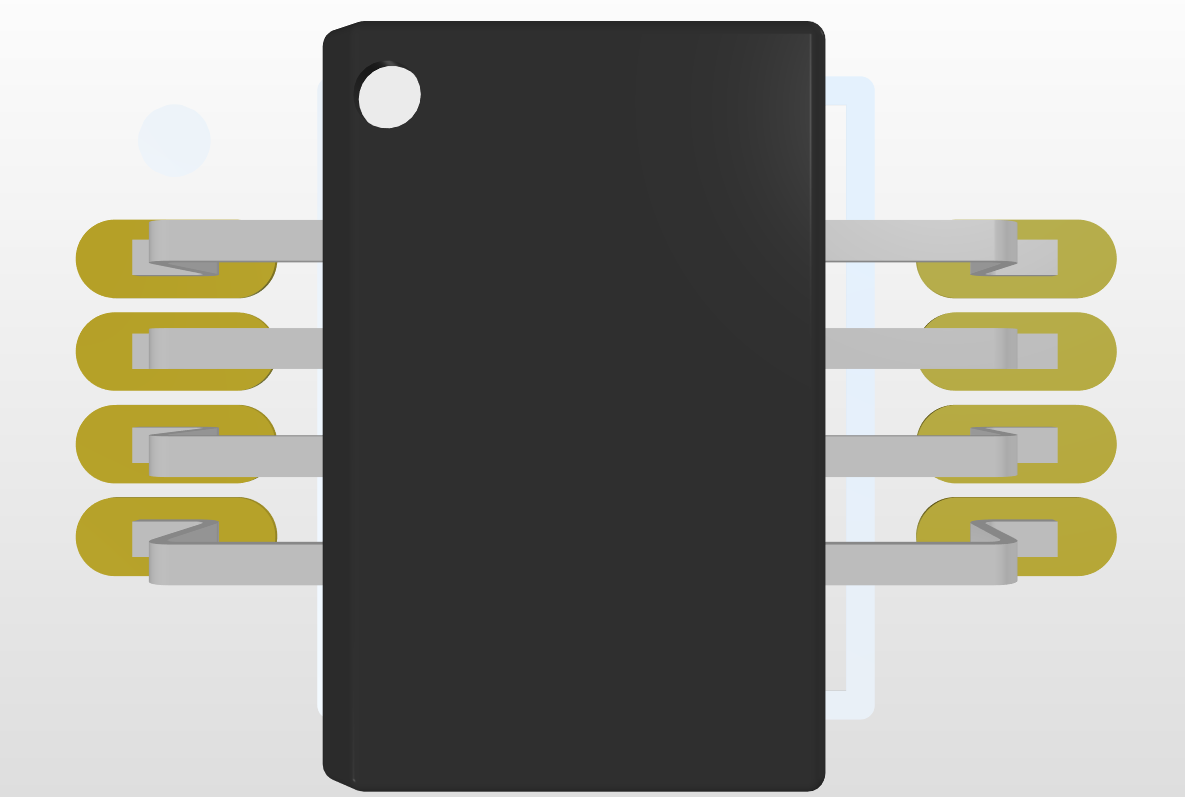
\includegraphics[width=0.9\textwidth]{pictures/ch3.11b.png}
            \caption{Mô hình PCB 3D LM358 SOP8 vừa tạo}
        \end{figure}
        \cleardoublepage
    \section{Add thư viện schematic và thư viện PCB lại với nhau}
        Bước 1: Ở màn hình làm việc của thư viện schematic chọn Add Footprint.
        \begin{figure}[H]
            \centering
            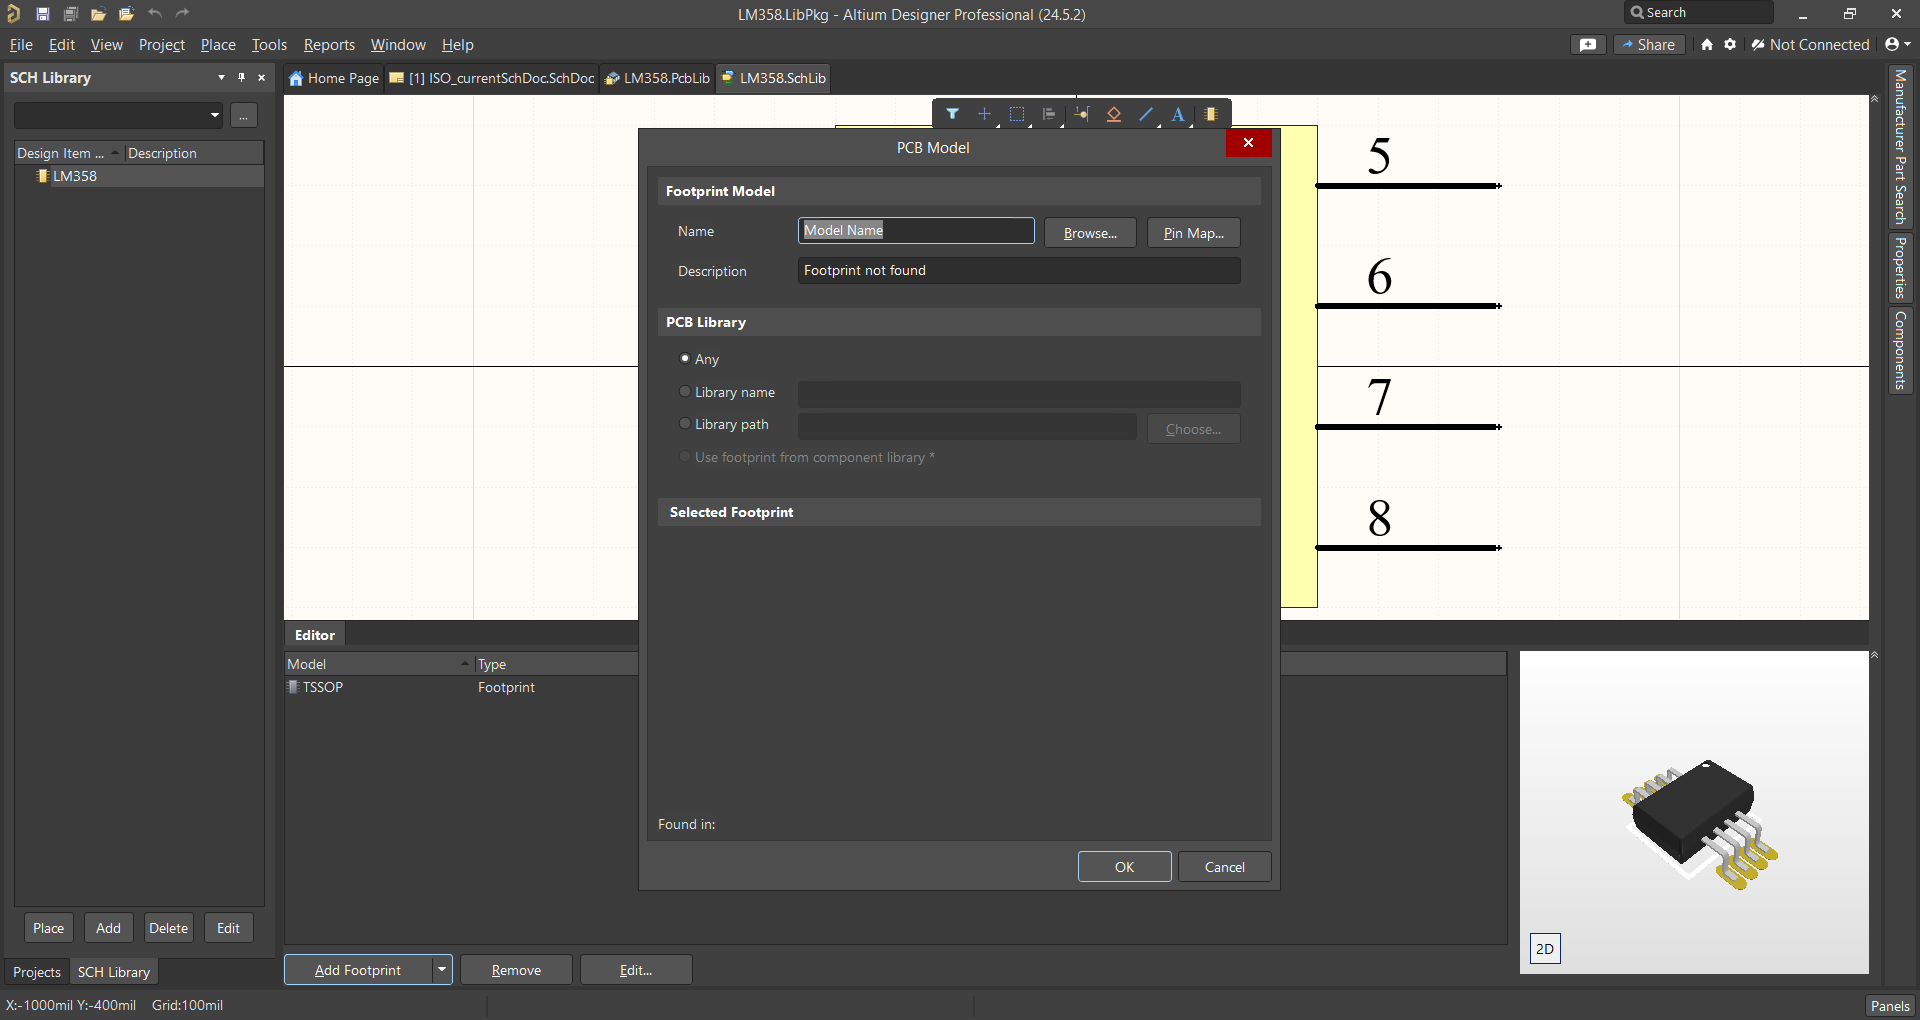
\includegraphics[width=1\textwidth]{pictures/ch3.12.png}
        \end{figure}
        Bước 2: Chọn Browse và chọn thư viện PCB tương ứng và nhấn OK
        \begin{figure}[H]
            \centering
            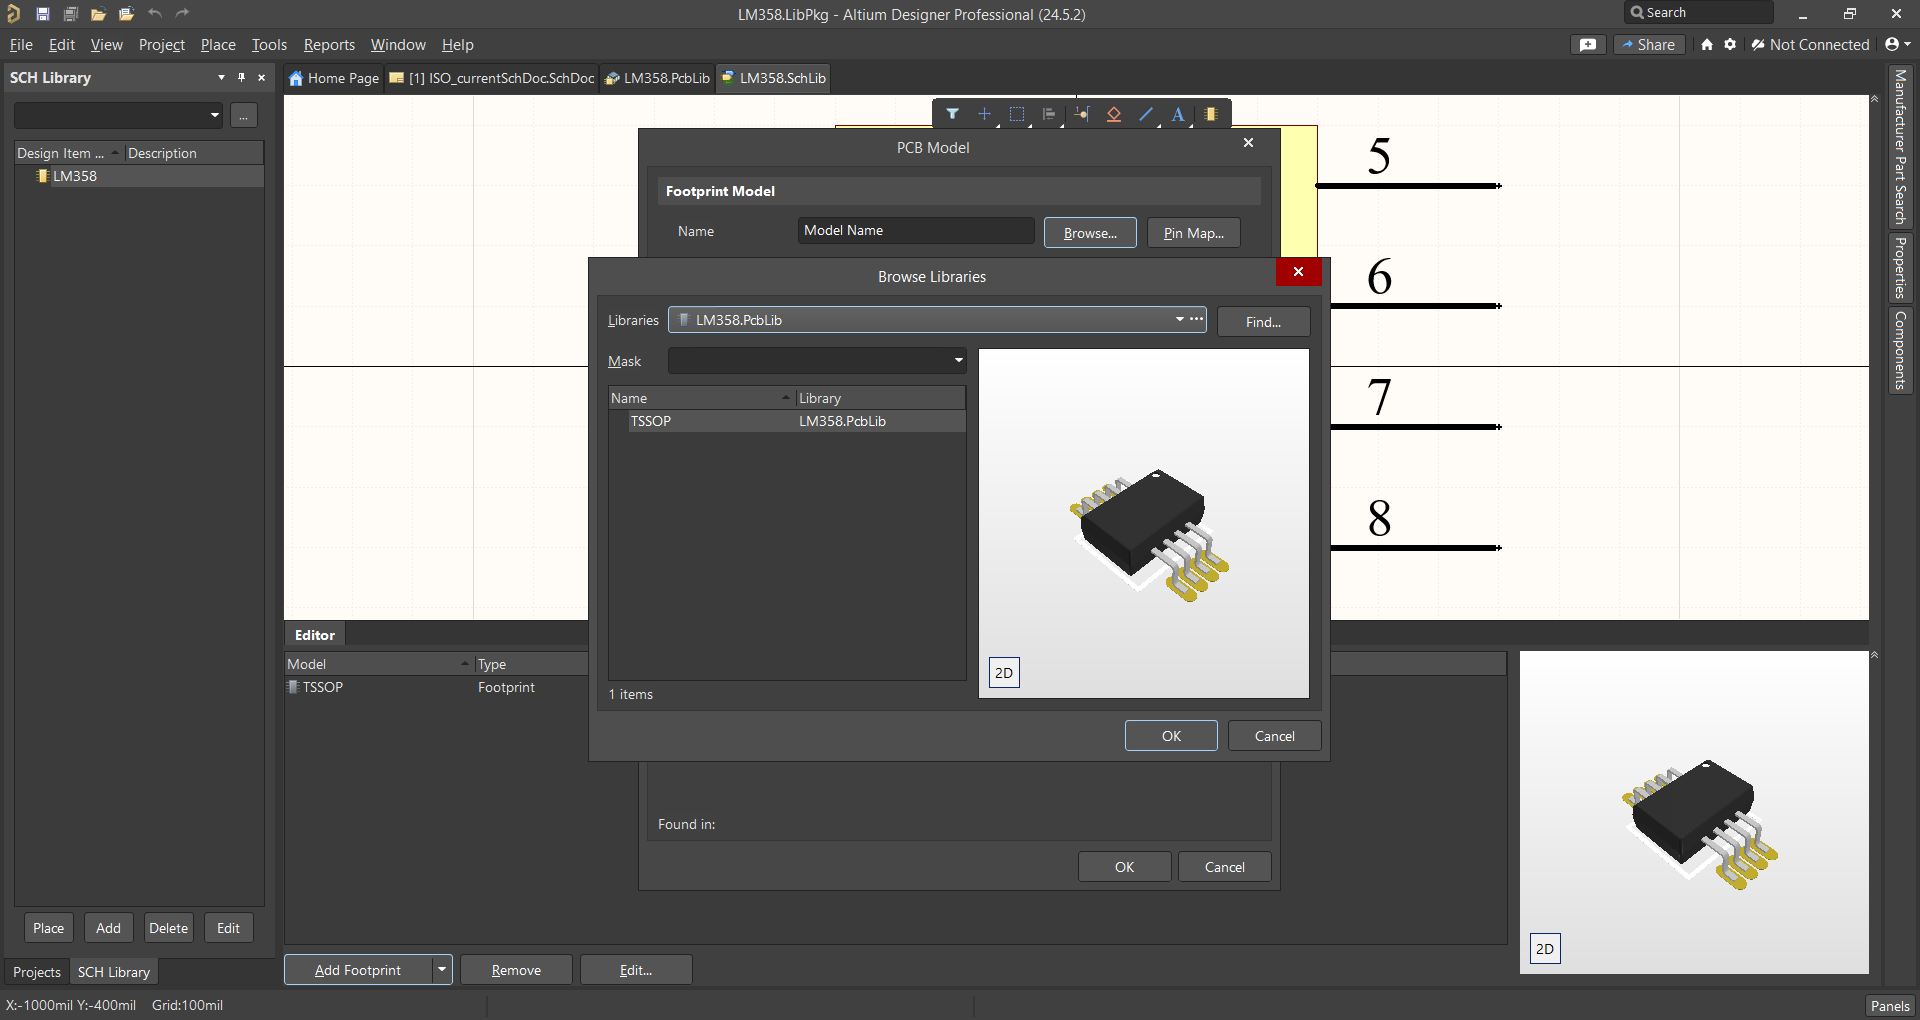
\includegraphics[width=1\textwidth]{pictures/ch3.13.png}
        \end{figure}
        \cleardoublepage
        Bước 3: Vào File/New chọn Library và chọn Integrated Library.
        \begin{figure}[H]
            \centering
            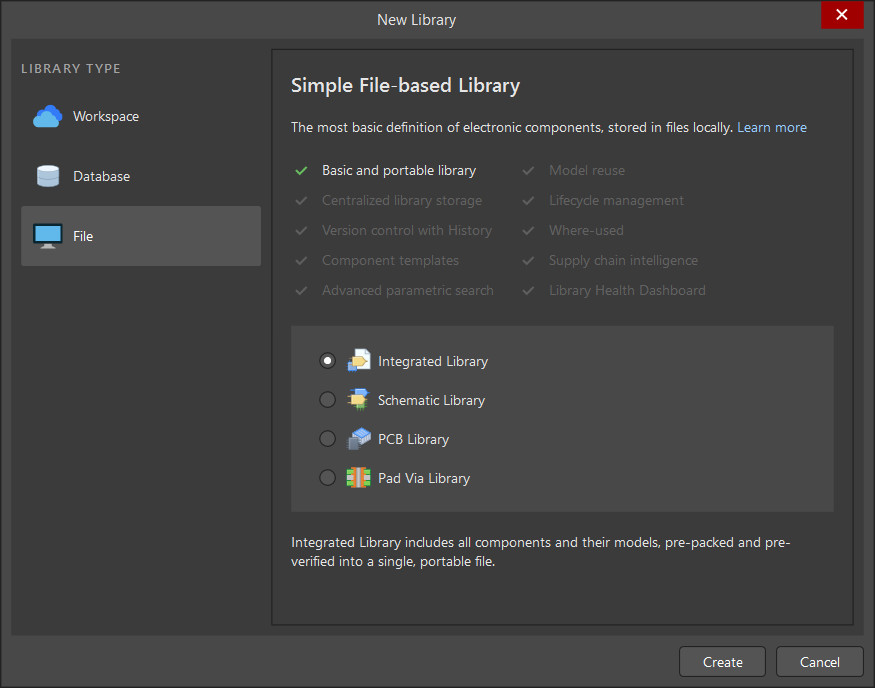
\includegraphics[width=1\textwidth]{pictures/ch3.15.png}
        \end{figure}
        Bước 4: Kéo 2 thư viện schematic và PCB vào Integrated Library vừa tạo và lưu lại. 
        Bước 5: Click chuột phải và chọn Compile Integrated Library.
        \begin{figure}[H]
            \centering
            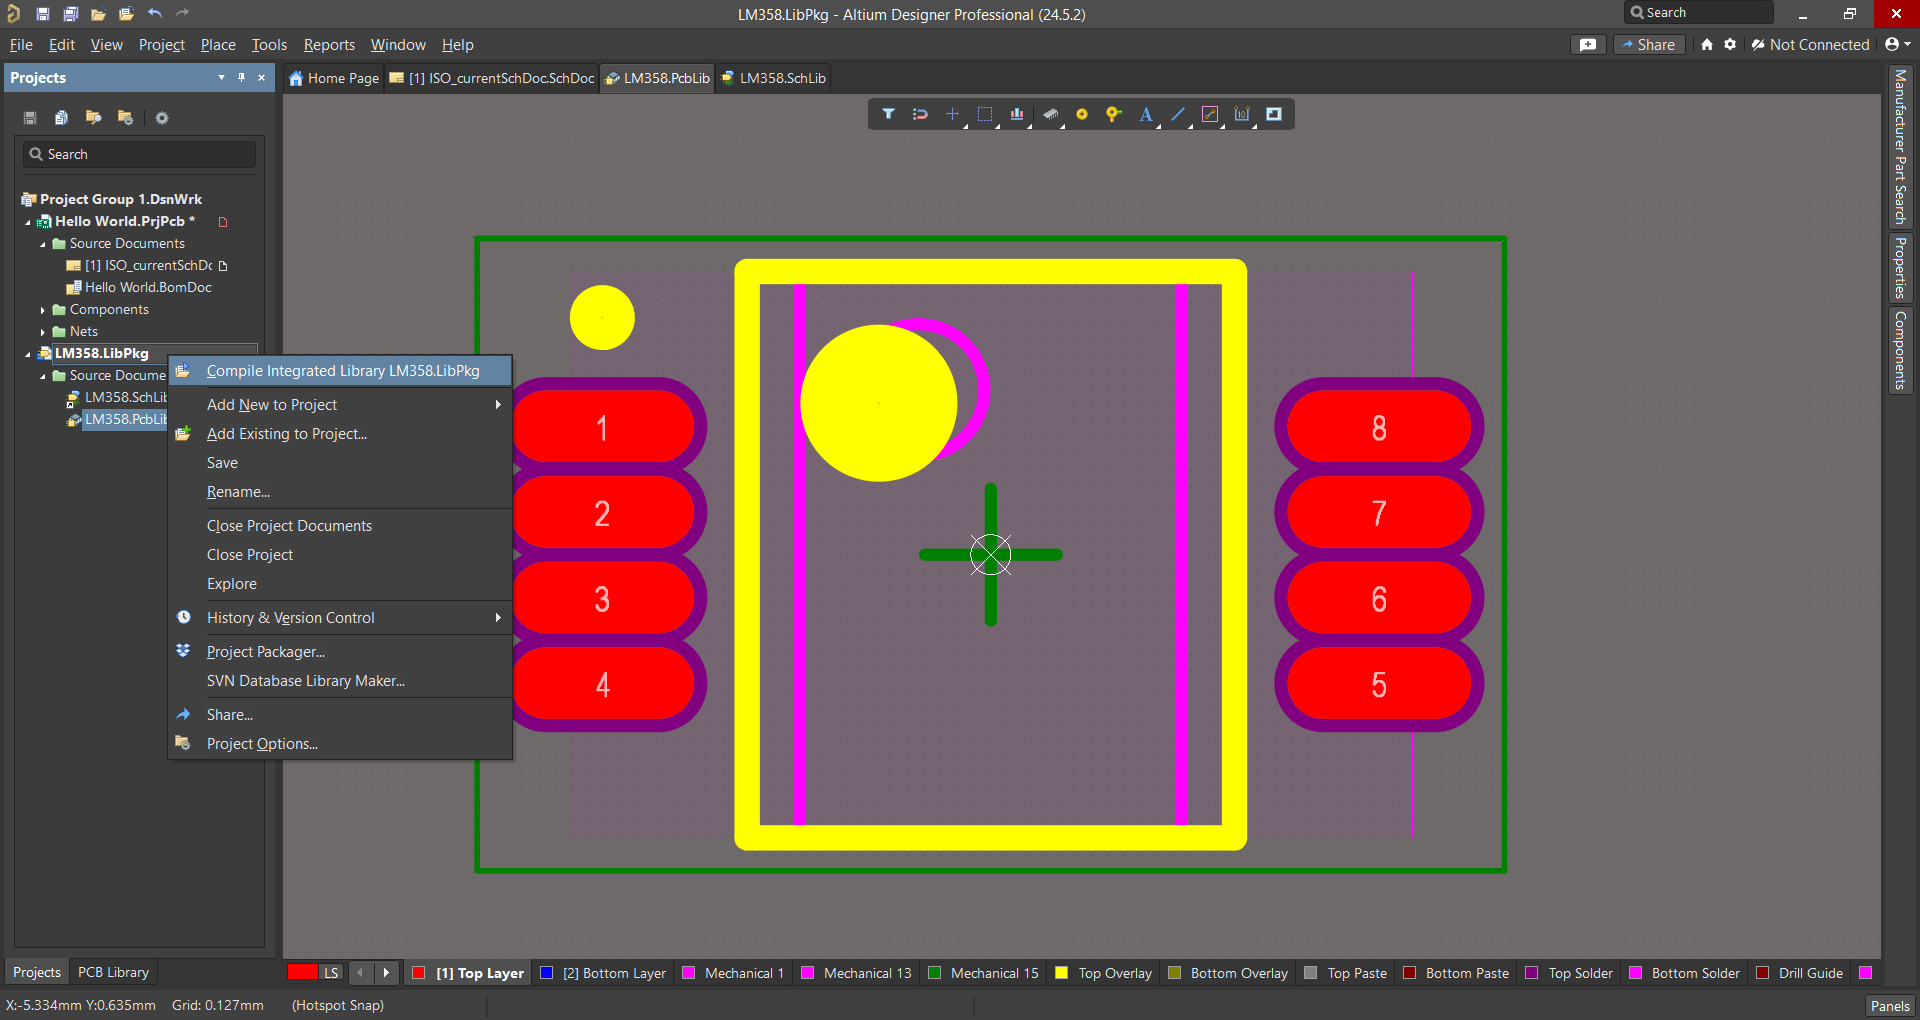
\includegraphics[width=1\textwidth]{pictures/ch3.16.png}
        \end{figure}
        \begin{figure}[H]
            \centering
            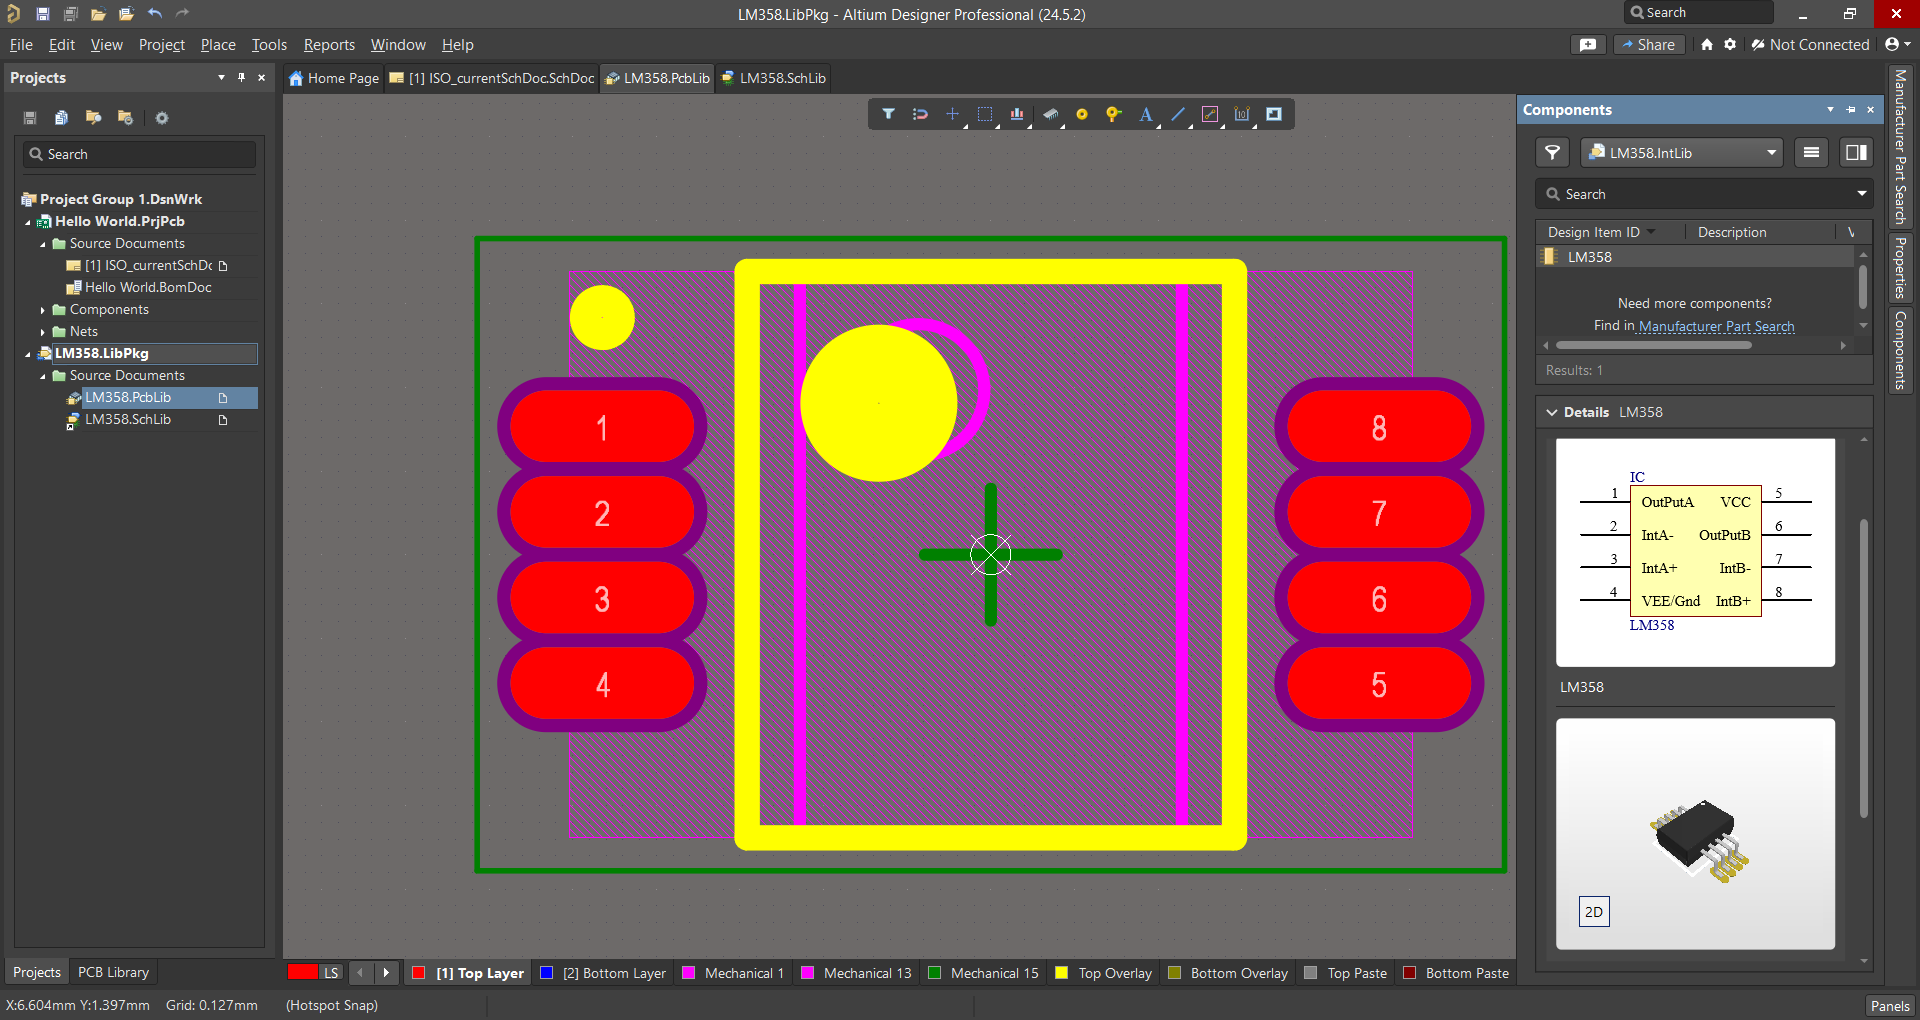
\includegraphics[width=1\textwidth]{pictures/ch3.14.png}
            \caption{Hoàn tất việc tạo thư viện schematic và PCB 3D cho LM358} 
        \end{figure}
        \cleardoublepage